%  LaTeX support: latex@mdpi.com 
%  For support, please attach all files needed for compiling as well as the log file, and specify your operating system, LaTeX version, and LaTeX editor.

%=================================================================
\documentclass[entropy,article,submit,moreauthors,pdftex]{Definitions/mdpi} 

% For posting an early version of this manuscript as a preprint, you may use "preprints" as the journal and change "submit" to "accept". The document class line would be, e.g., \documentclass[preprints,article,accept,moreauthors,pdftex]{mdpi}. This is especially recommended for submission to arXiv, where line numbers should be removed before posting. For preprints.org, the editorial staff will make this change immediately prior to posting.

%--------------------
% Class Options:
%--------------------
%----------
% journal
%----------
% Choose between the following MDPI journals:
% acoustics, actuators, addictions, admsci, adolescents, aerospace, agriculture, agriengineering, agronomy, ai, algorithms, allergies, analytica, animals, antibiotics, antibodies, antioxidants, appliedchem, applmech, applmicrobiol, applnano, applsci, arts, asi, atmosphere, atoms, audiolres, automation, axioms, batteries, bdcc, behavsci, beverages, biochem, bioengineering, biologics, biology, biomechanics, biomedicines, biomedinformatics, biomimetics, biomolecules, biophysica, biosensors, biotech, birds, bloods, brainsci, buildings, businesses, cancers, carbon, cardiogenetics, catalysts, cells, ceramics, challenges, chemengineering, chemistry, chemosensors, chemproc, children, civileng, cleantechnol, climate, clinpract, clockssleep, cmd, coatings, colloids, compounds, computation, computers, condensedmatter, conservation, constrmater, cosmetics, crops, cryptography, crystals, curroncol, cyber, dairy, data, dentistry, dermato, dermatopathology, designs, diabetology, diagnostics, digital, disabilities, diseases, diversity, dna, drones, dynamics, earth, ebj, ecologies, econometrics, economies, education, ejihpe, electricity, electrochem, electronicmat, electronics, encyclopedia, endocrines, energies, eng, engproc, entropy, environments, environsciproc, epidemiologia, epigenomes, fermentation, fibers, fire, fishes, fluids, foods, forecasting, forensicsci, forests, fractalfract, fuels, futureinternet, futuretransp, futurepharmacol, futurephys, galaxies, games, gases, gastroent, gastrointestdisord, gels, genealogy, genes, geographies, geohazards, geomatics, geosciences, geotechnics, geriatrics, hazardousmatters, healthcare, hearts, hemato, heritage, highthroughput, histories, horticulturae, humanities, hydrogen, hydrology, hygiene, idr, ijerph, ijfs, ijgi, ijms, ijns, ijtm, ijtpp, immuno, informatics, information, infrastructures, inorganics, insects, instruments, inventions, iot, j, jcdd, jcm, jcp, jcs, jdb, jfb, jfmk, jimaging, jintelligence, jlpea, jmmp, jmp, jmse, jne, jnt, jof, joitmc, jor, journalmedia, jox, jpm, jrfm, jsan, jtaer, jzbg, kidney, land, languages, laws, life, liquids, literature, livers, logistics, lubricants, machines, macromol, magnetism, magnetochemistry, make, marinedrugs, materials, materproc, mathematics, mca, measurements, medicina, medicines, medsci, membranes, metabolites, metals, metrology, micro, microarrays, microbiolres, micromachines, microorganisms, minerals, mining, modelling, molbank, molecules, mps, mti, nanoenergyadv, nanomanufacturing, nanomaterials, ncrna, network, neuroglia, neurolint, neurosci, nitrogen, notspecified, nri, nursrep, nutrients, obesities, oceans, ohbm, onco, oncopathology, optics, oral, organics, osteology, oxygen, parasites, parasitologia, particles, pathogens, pathophysiology, pediatrrep, pharmaceuticals, pharmaceutics, pharmacy, philosophies, photochem, photonics, physchem, physics, physiolsci, plants, plasma, pollutants, polymers, polysaccharides, proceedings, processes, prosthesis, proteomes, psych, psychiatryint, publications, quantumrep, quaternary, qubs, radiation, reactions, recycling, regeneration, religions, remotesensing, reports, reprodmed, resources, risks, robotics, safety, sci, scipharm, sensors, separations, sexes, signals, sinusitis, smartcities, sna, societies, socsci, soilsystems, solids, sports, standards, stats, stresses, surfaces, surgeries, suschem, sustainability, symmetry, systems, taxonomy, technologies, telecom, textiles, thermo, tourismhosp, toxics, toxins, transplantology, traumas, tropicalmed, universe, urbansci, uro, vaccines, vehicles, vetsci, vibration, viruses, vision, water, wevj, women, world 

%---------
% article
%---------
% The default type of manuscript is "article", but can be replaced by: 
% abstract, addendum, article, book, bookreview, briefreport, casereport, comment, commentary, communication, conferenceproceedings, correction, conferencereport, entry, expressionofconcern, extendedabstract, datadescriptor, editorial, essay, erratum, hypothesis, interestingimage, obituary, opinion, projectreport, reply, retraction, review, perspective, protocol, shortnote, studyprotocol, systematicreview, supfile, technicalnote, viewpoint, guidelines, registeredreport, tutorial
% supfile = supplementary materials

%----------
% submit
%----------
% The class option "submit" will be changed to "accept" by the Editorial Office when the paper is accepted. This will only make changes to the frontpage (e.g., the logo of the journal will get visible), the headings, and the copyright information. Also, line numbering will be removed. Journal info and pagination for accepted papers will also be assigned by the Editorial Office.

%------------------
% moreauthors
%------------------
% If there is only one author the class option oneauthor should be used. Otherwise use the class option moreauthors.

%---------
% pdftex
%---------
% The option pdftex is for use with pdfLaTeX. If eps figures are used, remove the option pdftex and use LaTeX and dvi2pdf.

%%%% ДЛЯ РУССКОГО ТЕКСТА закомментировать потом!
\usepackage{inputenc}
\usepackage[T2A,T1]{fontenc}
\usepackage[english,russian]{babel}
\usepackage{cmap}
%%%%


%=================================================================
% MDPI internal commands
\firstpage{1} 
\makeatletter 
\setcounter{page}{\@firstpage} 
\makeatother
\pubvolume{1}
\issuenum{1}
\articlenumber{0}
\pubyear{2021}
\copyrightyear{2020}
%\externaleditor{Academic Editor: Firstname Lastname} % For journal Automation, please change Academic Editor to "Communicated by"
\datereceived{} 
\dateaccepted{} 
\datepublished{} 
\hreflink{https://doi.org/} % If needed use \linebreak
%------------------------------------------------------------------
% The following line should be uncommented if the LaTeX file is uploaded to arXiv.org
%\pdfoutput=1

%=================================================================
% Add packages and commands here. The following packages are loaded in our class file: fontenc, inputenc, calc, indentfirst, fancyhdr, graphicx, epstopdf, lastpage, ifthen, lineno, float, amsmath, setspace, enumitem, mathpazo, booktabs, titlesec, etoolbox, tabto, xcolor, soul, multirow, microtype, tikz, totcount, changepage, paracol, attrib, upgreek, cleveref, amsthm, hyphenat, natbib, hyperref, footmisc, url, geometry, newfloat, caption

%=================================================================
%% Please use the following mathematics environments: Theorem, Lemma, Corollary, Proposition, Characterization, Property, Problem, Example, ExamplesandDefinitions, Hypothesis, Remark, Definition, Notation, Assumption
%% For proofs, please use the proof environment (the amsthm package is loaded by the MDPI class).

%=================================================================
% Full title of the paper (Capitalized)
\Title{Ускорение метода глобальной оптимизации за счет выделения локальных экстремумов на основе машинного обучения}
%		   Acceleration of Global Optimization Algorithm by Detecting Local Extrema Based on Machine Learning

% MDPI internal command: Title for citation in the left column
\TitleCitation{}

% Author Orchid ID: enter ID or remove command
\newcommand{\orcidauthorA}{0000-0001-5273-2471} % Add \orcidA{} behind the author's name
\newcommand{\orcidauthorB}{0000-0002-8736-0652} % Add \orcidB{} behind the author's name
\newcommand{\orcidauthorC}{0000-0002-4013-2329} % Add \orcidB{} behind the author's name

% Authors, for the paper (add full first names)
\Author{Konstantin Barkalov $^{1}$*\orcidA{} and Ilya Lebedev $^{1}$\orcidB{}}

% MDPI internal command: Authors, for metadata in PDF
\AuthorNames{Konstantin Barkalov and Ilya Lebedev}

% MDPI internal command: Authors, for citation in the left column
\AuthorCitation{Barkalov, K.; Lebedev, I.}
% If this is a Chicago style journal: Lastname, Firstname, Firstname Lastname, and Firstname Lastname.

% Affiliations / Addresses (Add [1] after \address if there is only one affiliation.)
\address[1]{%
$^{1}$ \quad Department of Mathematical Software and Supercomputing Technologies, Lobachevsky University, 603950 Nizhni Novgorod, Russia; ilya.lebedev@itmm.unn.ru (I.L.)}
%$^{2}$ \quad Affiliation 2; e-mail@e-mail.com}

% Contact information of the corresponding author
\corres{Correspondence: konstantin.barkalov@itmm.unn.ru (K.B.)}
%; Tel.: (optional; include country code; if there are multiple corresponding authors, add author initials) +xx-xxxx-xxx-xxxx (F.L.)}

% Current address and/or shared authorship
%\firstnote{Current address: Affiliation 3} 
%\secondnote{These authors contributed equally to this work.}
% The commands \thirdnote{} till \eighthnote{} are available for further notes

%\simplesumm{} % Simple summary

%\conference{} % An extended version of a conference paper

% Abstract (Do not insert blank lines, i.e. \\) 
\abstract{
В статье рассматриваются задачи глобальной оптимизации и численные методы их решения. Задачи указанного класса являются вычислительно-трудоемкими, т.к. целевая функция может являться многоэкстремальной, недифференцируемой, и, как правильно, заданной в виде «черного ящика». В проведенном исследовании использовался детерминированный алгоритм поиска глобального экстремума, который не основан на идеях мультистарта и nature-inspired algorithms. В статье приведены вычислительные правила одномерного алгоритма и nested optimization scheme, которая позволяет применять его для решения сложных многомерных задач. Отметим, что сложность решения задач глобальной оптимизации существенным образом зависит от наличия многих локальных экстремумов. В работе предложен алгоритм выделения областей притяжения локальных минимумов, основанный на использовании методов машинного обучения (в частности, деревьев решений). Использование в выделенных областях алгоритмов локальной оптимизации позволяет значительно ускорить сходимость глобального поиска за счет снижения числа поисковых испытании в окрестностях локальных минимумов. Приведены результаты вычислительных экспериментов, проведенных на нескольких сотнях задач глобальной оптимизации разной размерности, которые подтверждают эффект ускорения сходимости (в терминах числа поисковых испытаний, требующихся для решения задачи с заданной точностью).
}

% Keywords
\keyword{global optimization; local optimization; multiextremal problems; numerical methods; approximation; decision trees} 

% The fields PACS, MSC, and JEL may be left empty or commented out if not applicable
%\PACS{J0101}
%\MSC{}
%\JEL{}

%%%%%%%%%%%%%%%%%%%%%%%%%%%%%%%%%%%%%%%%%%
% Only for the journal Diversity
%\LSID{\url{http://}}

%%%%%%%%%%%%%%%%%%%%%%%%%%%%%%%%%%%%%%%%%%
% Only for the journal Applied Sciences:
%\featuredapplication{Authors are encouraged to provide a concise description of the specific application or a potential application of the work. This section is not mandatory.}
%%%%%%%%%%%%%%%%%%%%%%%%%%%%%%%%%%%%%%%%%%

%%%%%%%%%%%%%%%%%%%%%%%%%%%%%%%%%%%%%%%%%%
% Only for the journal Data:
%\dataset{DOI number or link to the deposited data set in cases where the data set is published or set to be published separately. If the data set is submitted and will be published as a supplement to this paper in the journal Data, this field will be filled by the editors of the journal. In this case, please make sure to submit the data set as a supplement when entering your manuscript into our manuscript editorial system.}

%\datasetlicense{license under which the data set is made available (CC0, CC-BY, CC-BY-SA, CC-BY-NC, etc.)}

%%%%%%%%%%%%%%%%%%%%%%%%%%%%%%%%%%%%%%%%%%
% Only for the journal Toxins
%\keycontribution{The breakthroughs or highlights of the manuscript. Authors can write one or two sentences to describe the most important part of the paper.}

%%%%%%%%%%%%%%%%%%%%%%%%%%%%%%%%%%%%%%%%%%
% Only for the journal Encyclopedia
%\encyclopediadef{Instead of the abstract}
%\entrylink{The Link to this entry published on the encyclopedia platform.}
%%%%%%%%%%%%%%%%%%%%%%%%%%%%%%%%%%%%%%%%%%
\begin{document}
%%%%%%%%%%%%%%%%%%%%%%%%%%%%%%%%%%%%%%%%%%

\section{Introduction}

%The introduction should briefly place the study in a broad context and highlight why it is important. It should define the purpose of the work and its significance. The current state of the research field should be reviewed carefully and key publications cited. Please highlight controversial and diverging hypotheses when necessary. Finally, briefly mention the main aim of the work and highlight the principal conclusions. As far as possible, please keep the introduction comprehensible to scientists outside your particular field of research. Citing a journal paper \cite{ref-journal}. Now citing a book reference \cite{ref-book1,ref-book2} or other reference types \cite{ref-unpublish,ref-communication,ref-proceeding}. Please use the command \citep{ref-thesis,ref-url} for the following MDPI journals, which use author--date citation: Administrative Sciences, Arts, Econometrics, Economies, Genealogy, Histories, Humanities, IJFS, Journal of Intelligence, Journalism and Media, JRFM, Languages, Laws, Religions, Risks, Social Sciences.

Успешное применение методов машинного обучения (ML) для решения широкого спектра задач приводит к созданию новых подходов к эффективному использованию идей ML в различных областях приложений. 
Примером класса задач, в которых методы машинного обучения продемонстрировали свою эффективность, являются задачи выявления основных свойств исследуемых явлений (например, физических, экономических или социальных), которые характеризуются стохастической природой или наличием скрытых параметров \cite{Golovenkin2020,Gonoskov2019}.
Методы машинного обучения успешно используются и для решения сложных задач вычислительной математики, например, для simulation of dynamical systems \cite{Seleznev2019}, решения ordinary, partial or stochastic differential equations \cite{Lagaris1998,Blechschmidt2021,Xu2020} .

Одной из таких сложных задач вычислительной математики, к решению которой можно так или иначе применить методы машинного обучения, являются задачи глобальной оптимизации. 
В таких задачах, как правило, не представляется возможным найти решение аналитически и возникает необходимость построения численных методов для его поиска.

Проблема численного решения задач оптимизации сопряжена со значительными трудностями. Во многом они связаны с размерностью и видом целевой функции. При этом наиболее сложными являются задачи, в которых целевая функция является многоэкстремальной, недифференцируемой и, более того, заданной в форме черного ящика (т. е. в виде некоторой вычислительной процедуры, на вход которой подается аргумент, а выходом является соответствующее значение функции). Методы решения именно таких задач рассматриваются в данной статье. 

Можно выделить несколько подходов к построению численных методов решения задач глобальной оптимизации. 
%Надо ли добавить алгоритмы на основе метамоделей ?
Ряд алгоритмов основан на идее мультистарта: запуск локального поиска либо начиная с разных стартовых точек, либо с использованием разных параметров. Методы локальной оптимизации обладают большой скоростью сходимости. При этом одной из основных проблем в мультистартовых схемах является выбор начальных точек, которые бы соответствовали областям притяжения различных локальных решений. 
К решению данной проблемы могут быть успешно применены методы машинного обучения. 
Например, в \cite{RinnooyKan1987} для выбора перспективных стартовых точек использовались методы кластерного анализа. 
В \cite{Cassioli2012} область для запуска локального метода выделялась на основе классификации стартовых точке с помощью support vector machine.

Еще одним популярным классом методов, применимым к решению задач глобальной оптимизации, являются метаэвристические алгоритмы. 
Многие из них основаны на имитации процессов, протекающих в живой природе. Для настройки параметров таких алгоритмов также применимы методы машинного обучения. Например, в \cite{Jin2005} приведен обзор использования методов машинного обучения в эволюционных алгоритмах.

Следует отметить, что алгоритмы последних двух классов не обеспечивают гарантированную сходимость к решению задачи и проигрывают детерминированным алгоритмам по качеству работы \cite{Kvasov2018,Sergeyev2018} (e.g., measured by the number of correctly solved problems from a certain set). Поэтому перспективным является использование именно детерминированных методов.


One of the efficient deterministic methods for solving multiextremal optimization problems is \textit{the information-statistical global search algorithm} \cite{Strongin2000}. This method initially proposed for solving unconstrained optimization problems was successfully generalized to the classes of optimization problems with non-convex constraints and multicriteria optimization problems. For different versions of the algorithm, parallelization methods taking into account the architecture of modern computing systems were also suggested \cite{Barkalov2016,globalizerSystem,Strongin2018}.


Для алгоритма глобального поиска в разное время было предложено несколько стратегий ускорения его работы (в терминах числа итераций, требующихся для решения задачи с заданной точностью). В данной работе предлагается новый подход к ускорению, основанный на выявления областей притяжения локальных минимумов с использованием методов машинного обучения. Выявление областей притяжения и запуск в этих областях локального поиска позволяет существенным образом сократить число испытаний, требующееся методу для достижения глобальной сходимости. Сказанное подтверждается результатами экспериментов, проведенных на серии из нескольких сотен тестовых задач. 



\section{Problem Statement}

В данной работе мы будем рассматривать задачи глобальной оптимизации вида
\begin{eqnarray}\label{main_problem}
& \varphi(y^\ast)=\min{\left\{\varphi(y):y\in D\right\}},\\
& D=\left\{y\in \text{R}^N: a_i\leq y_i \leq b_i, 1\leq i \leq N\right\}. \nonumber
\end{eqnarray}
Задача (\ref{main_problem}) рассматривается в предположении, что целевая функция является многоэкстремальной, задана как ``черный ящик'', а вычисление ее значений связано с решением задачи численного моделирования и является трудоемкой операцией.

Для многих прикладных задач типичной является ситуация, когда ограниченное изменение вектора параметров $y$ вызывает ограниченное изменение значений $\varphi(y)$. Математической моделью, описывающей указанное предположение, является предположение о выполнимости условия Липшица
\[
\left|\varphi(y')-\varphi(y'')\right|\leq L\left\|y'-y''\right\|,\; y',y'' \in D,\; 0<L<\infty.
\]
Предположение липшицевости целевой функции типично для многих подходов к разработке оптимизационных алгоритмов \cite{Jones1993,Pinter1996,Zilinskas2008,Evtushenko2009}.
При этом многие известные методы основаны на различных способах разбиения области поиска на систему подобластей и последующего выбора наиболее перспективной подобласти для размещения очередного испытания (вычисления значения целевой функции) \cite{Jones2009,Zilinskas2010,Evtushenko2013,Kvasov2013,Paulavicius2016}. 

Важным свойством задач глобальной оптимизации является тот факт, что в отличие от задач на поиск локального экстремума, глобальный минимум является интегральной характеристикой решаемой задачи. Чтобы убедиться, что точка $y^*\in D$ является решением задачи, недостаточно исследовать лишь ее окрестность, требуется исследование всей области поиска. Как результат, при минимизации существенно многоэкстремальных функций численный метод должен построить покрытие области поиска и число узлов этого покрытия увеличивается экспоненциально с ростом размерности. 
Эта особенность обуславливает высокую трудоемкость решения задач многоэкстремальной оптимизации, и размерность является решающим фактором, влияющим на сложность их решения. 

Для преодоления сложностей, вызванных размерностью решаемой задачи, в многоэкстремальной оптимизации широко используются различные подходы к уменьшению размерности.  
Например, simplicial or diagonal partition области поиска позволяет использовать для решения исходной многомерной задачи методы решения одномерных задач (see, for example, \cite{PaulaviciusZilinskas2014,Sergeyev2017,Sergeyev2013}). 
Известным подходом к редукции размерости является также использование Peano space-filling curves mapping the multidimensional domain onto one-dimensional interval \cite{Strongin2000}.

В данной работе мы будем использовать еще один способ, основанный на the nested optimization scheme \cite{Shi2000,Grishagin2001,VanDam2010,Grishagin2015} and in its generalization \cite{Grishagin2016,Grishagin2016_1}.
The nested optimization scheme, с одной стороны, не ухудшает свойств минимизируемой функции (в отличие от редукции с использованием Peano curves), а с другой стороны, не требует использования сложных структур данных для поддержки симплексных или диагональных разбиений допустимой области. 
Одновременно с этим схема вложенной оптимизации позволяет свести решение многомерной задачи к решению набора стандартных одномерных задач и использовать широкий спектр алгоритмов одномерной глобальной оптимизации для их решения.

\section{Methods}

\subsection{Core global search algorithm}\label{CoreGSA}

В качестве стандартной задачи рассмотрим одномерную задачу многоэкстремальной оптимизации 
\begin{equation}\label{uni_problem}
\varphi^\ast = \varphi(x^\ast)=\min{\left\{\varphi(x):x\in \left[0,1\right] 
\right\}}
\end{equation}
с целевой функцией, удовлетворяющей условию Липшица.

Приведем описание global search algorithm (GSA) для решения базовой задачи в соответствии с \cite{Strongin2000}.
В процессе своей работы GSA порождает последовательность точек $x^i$, в которых вычисляются значения целевой функции $z^i=\varphi(x^i)$. 
Будем называть процесс вычисления значения целевой функции \textit{trial}.

В соответствии с алгоритмом первые два испытания проводятся в граничных точках отрезка $[0,1]$, т.е. $x^0=0,\;x^1=1$. 
В этих точках вычисляются значения целевой функции $z^0=\varphi(x^0),\;z^1=\varphi(x^1)$ и устанавливается значение счетчика $k=1$. 
Точка очередного испытания $x^{k+1}, k\geq 1,$ выбирается в соответствии со следующими действиями.

 Step 1. Перенумеровать нижним индексом (начиная с 0) точки $x^i,\:0\leq i\leq k$, проведенных испытаний в порядке возрастания координаты, т.е.
\begin{equation}\label{xt}
0=x_0<x_1<\ldots <x_{k}=1.
\end{equation} 
Сопоставить точкам $x_i, \; 0\leq i\leq k$, вычисленные в них значения целевой функции $z_i=\varphi(x_i), \; 0\leq i\leq k$.

Step 2. Вычислить максимальное абсолютное значение относительной первой разности
\begin{equation}\label{mu}
\mu=\max_{1\leq i\leq k}\frac{\left|z_i-z_{i-1}\right|}{\Delta_i},
\end{equation}
где $\Delta_i = x_i-x_{i-1}$. Если вычисленное в соответствии с данной формулой значение равно нулю, то положить $\mu = 1$.

Step 3. Для всех интервалов $(x_{i-1},x_i),1\leq i\leq k$,  вычислить значение
\begin{equation}\label{R}
R(i)=r\mu\Delta_i+\frac{(z_i-z_{i-1})^2}{r\mu\Delta_i}-2(z_i+z_{i-1}),
\end{equation} 
называемое \textit{характеристикой} интервала; величина $r>1$ является параметром алгоритма. 

Step 4. Найти интервал $(x_{t-1},x_t)$ с максимальной характеристикой
\begin{equation}\label{MaxR}
R(t)=\max_{1\leq i\leq {k}}R(i).
\end{equation}
Если максимальная характеристика соответствует нескольким интервалам, то в качестве $t$ выбрать минимальное число, удовлетворяющее (\ref{MaxR}).

Step 5. Провести новое испытание в точке
\begin{equation}\label{xk1}
x^{k+1}=\frac{1}{2}(x_{t-1}+x_t) - \frac{z_t-z_{t-1}}{2r\mu}.
\end{equation}

Алгоритм прекращает свою работу при выполнении условия $\Delta_t<\epsilon$; здесь $t$ из (\ref{MaxR}), а $\epsilon>0$ есть заданная точность. 
В качестве оценки решения задачи выбираются значения 
\[
z_k^\ast=\min_{0\leq i \leq k}\varphi(x^i), \ x_k^\ast=\arg \min_{0\leq i \leq
 k}\varphi(x^i).
\] 

Теоретические условия, определяющие сходимость алгоритма, представлены в \cite{Strongin2000}. 
Работа алгоритма при минимизации конкретной многоэкстремальной функции, которая задаются в соответствии с формулой (\ref{hill}), проиллюстрирована на figure \ref{fig1}. При запуске алгоритма использовался параметр $r=2.2$ из (\ref{R}) и значение $\epsilon = 10^{-3}$ в критерии остановки метода.
На рисунке \ref{fig1} изображен график objective function и точки 71 поискового испытания, потребовавшихся GSA для решения задачи с указанной точностью. Наглядно видна проблема всех методов глобальной оптимизации -- концентрация точек в окрестностях локальных минимумов задачи, которые не являются глобальным решением. 

\begin{figure}[H]
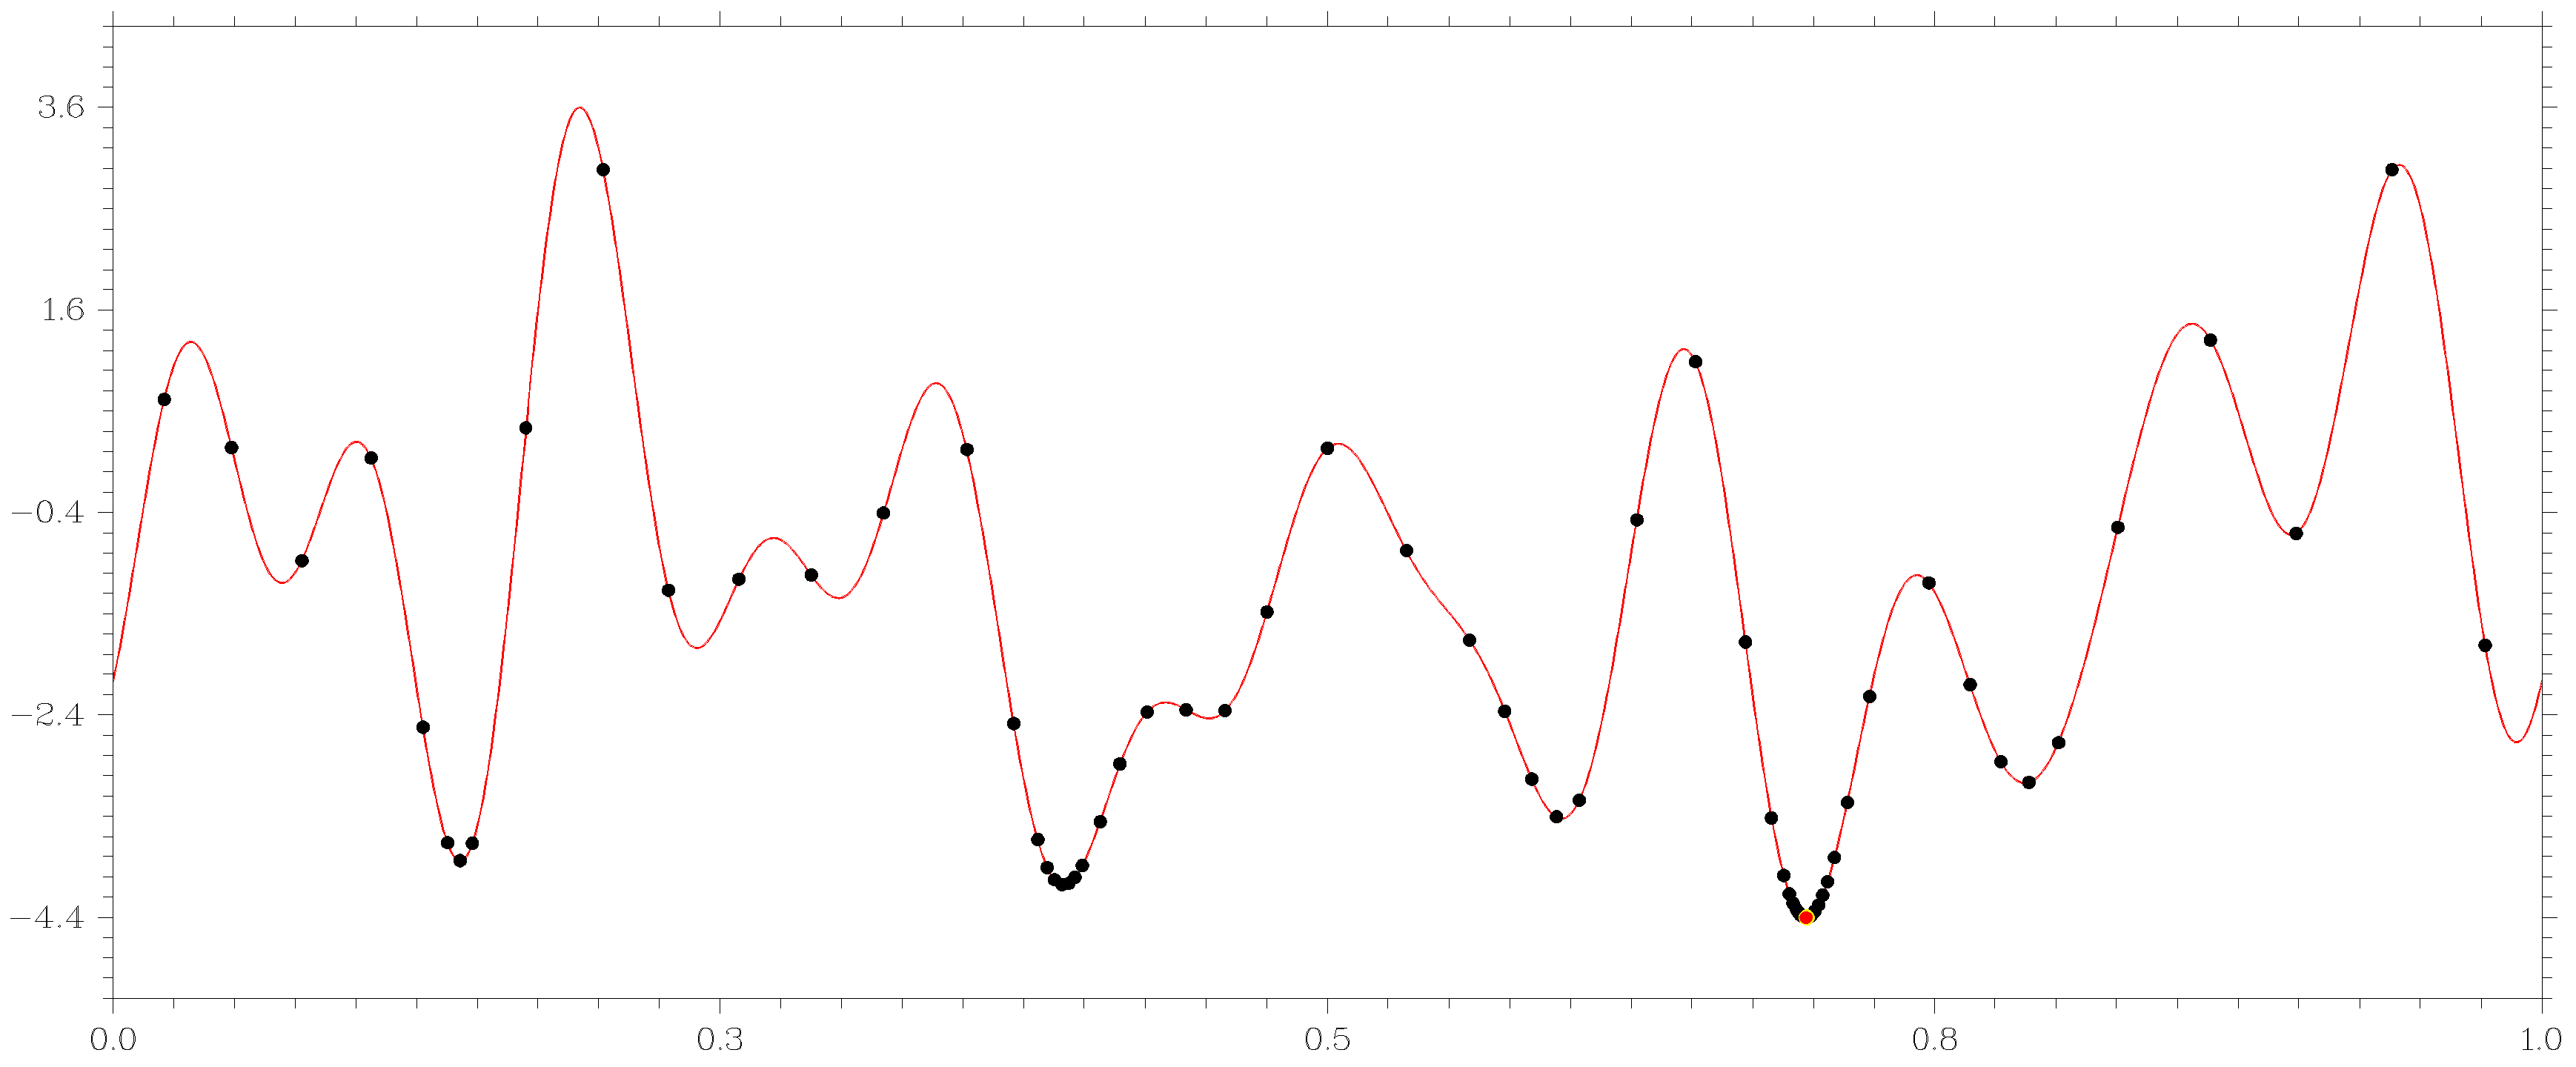
\includegraphics[width=1.0\linewidth]{HillAGP90.png}
\caption{Минимизация функции вида (\ref{hill}) с помощью GSA.}
\label{fig1}
\end{figure}   


\subsection{Machine Learning Regression как инструмент для выделения областей притяжения локальных экстремумов}\label{TreeGSA}

Функции, рассматриваемые в рамках данного исследования, принадлежат классу липшицевых функций. Поэтому классические методы регрессии (например, полиномиальная регрессия, когда функция приближается полиномом заданной степени) не будут хорошо соответствовать поведению функции. 

Более мощным инструментом являются регрессионные сплайны. При построении регрессионного сплайна область определения разбивается на $K$ непересекающихся подобластей, в каждой из которых функция аппроксимируется полиномом. При разбиении интервала на достаточное число подобластей позволяет очень точно аппроксимировать исходную функцию. 

Построить регрессию можно также и с использованием такого мощного инструмента, как искусственные нейронные сети. 
Для построения регрессии могут быть использованы сети разного типа, например, multilayer perceptron, radial basis function network, и т.д. 
Однако в обоих этих случаях модель (сплайн или же нейронная сеть) сама становится сложной для того анализа, который требуется выполнить в решаемой проблеме (выделение областей притяжения локальных экстремумов). 

Поэтому в рамках проведенного исследования для анализа локального поведения функции мы выбрали регрессионную модель, основанную на деревьях решений. 
Например, если целевая функция хорошо аппроксимируется полиномами, то полиномиальная регрессия, конечно же, будет адекватно передавать свойства функции. Однако если между имеет место более сложная зависимость, тогда дерево решений может превзойти по качеству аппроксимации классические варианты регрессии.
%Здесь нужен рисунок - функция Шекеля, и два варианта регрессии - полином и деревья решений. Шекель должен плохо полиномами представляться, т.к. там функции вида 1/x
Одновременно с этим регрессия на основе дерева решений позволяет с достаточной точностью легко выделять области притяжения локальных экстремумов.

Построение регрессии с помощью дерева решений включает два основных этапа:
\begin{itemize}
	\item Область поиска $D$ разбивается на $J$ непересекающихся подобластей $D_1, D_2, ..., D_J$, причем $D = \bigcup_{j=1}^{J}{D_j}$.
	\item Любому значению, попадающему в область $D_j$, т.е. $x \in D_j$, ставится в соответствие среднее значение $c_j$ по значениям training trials, попавших в эту область.
\end{itemize}

Фактически, деревья решений строят модель функции вида
\begin{equation}\label{dtree}
f(x) = c_j, \; x\in D_j.
\end{equation}
 
Указанная модель является, с одной стороны, довольно простой, а с другой стороны, адекватно отражает интересующие нас свойства функции (наличие или отсутствие локальных минимумов). Выделение областей притяжения локальных минимумов с использованием модели (\ref{dtree}) можно организовать следующим образом.

Пусть $x^{k+1}$ -- точка текущего испытания. Для данной точки ищется номер $j$, такой что $x^{k+1} \in D_j$. 
Далее сравниваются значения $c_j$, соответствующие соседним подобластям. Если выполняется одно из условий
\begin{gather}\label{LocalPointC}
c_{j} \leq c_{j+1} \leq c_{j+2} \leq c_{j+3} \leq c_{j+4}, \; j=1; \nonumber \\ 
c_{j-1} \geq c_{j} \leq c_{j+1} \leq c_{j+2} \leq c_{j+3}, \; j=2;  \nonumber \\  
c_{j-2} \geq c_{j-1} \geq c_{j} \leq c_{j+1} \leq c_{j+2}, \; 3 \leq j \leq J-2; \\ 
c_{j-3} \geq c_{j-2} \geq c_{j-1} \geq c_{j} \leq c_{j+1}, \; j=J-1; \nonumber \\ 
c_{j-4} \geq c_{j-3} \geq c_{j-2} \geq c_{j-1} \geq c_{j}, \; j=J; \nonumber 
\end{gather}
то область $D_j$ считается областью притяжения локального минимума. В ней можно запускать локальный поиск, а впоследствии -- исключить данную подобласть из глобального поиска.
В качестве локального алгоритма может использоваться любой из локальных методов нулевого порядка, например,  golden section search or parabolic interpolation \cite{Press}.

Для того, чтобы модифицировать алгоритм глобального поиска из subsection \ref{CoreGSA} с целью исключения областей притяжения локальных минимумов, сопоставим каждой точке испытания $x^i$, получаемой при работе алгоритма, дополнительный признак $q^i \in \{0,1,2\}$, который будет характеризовать свойства данной точки. 
Значение $q^i=0$ присваивается по умолчанию и означает что точка $x^i$ получена в результате работы правила (\ref{xk1}) алгоритма глобального поиска.
Значение $q^i=1$ присваивается точкам, полученным в результате работы локального метода, при этом значение $q^i=2$ соответствует точке локального минимума, найденной в результате работы локального поиска. 

Напомним, что верхний индекс соответствует номеру итерации, на которой было проведено испытание в данной точке, а нижний индекс -- номеру точки в ряду (\ref{xt}).

Опишем теперь модифицированный алгоритм глобального поиска, использующий деревья решений для выделения и исключения областей притяжения локальных минимумов; будем в дальнейшем ссылаться на данный алгоритм как на GSA-DT.

Шаги 1--5 алгоритма GSA-DT полностью повторяют шаги 1--5 . 

Step 6. Если $q_{t-1} \in \{1,2\}$ или $q_t \in \{1,2\}$, то перейти к проверке критерия остановки. Иначе перейти на Step 7.

Step 7. Построить дерево решений на основе результатов выполненных испытаний, и получить соответствующую кусочно линейную аппроксимацию, которая каждой подобласти $D_1, D_2, ..., D_J$ сопоставляет значение $c_1, c_2, ..., c_J$.

Step 8. Для точки $x^{k+1}$ текущего испытания найти номер $j$ такой, что $x^{k+1} \in D_j$ и проверить выполнимость условия (\ref{LocalPointC}). Если условие (\ref{LocalPointC}) выполняется, запустить в области $D_j$ локальный поиск из точки $x^{k+1}$. 
Результаты всех испытаний, выполненных в процессе работы локального поиска в точках $x^{k+2}, ...,x^{k+k_{local}}$, сохраняются в информационной базе алгоритма и используются на последующих итерациях. 
Все эти точки получают признак $q^i=1$, $i = k+2, ... , k+k_{local}$. Точке, соответствующей найденному локальному минимуму, присваивается признак равный 2.

Критерий остановки модифицированного алгоритма будет выглядеть следующим образом. 
Алгоритм прекращает свою работу при выполнении одного из условий:

\begin{itemize}
	\item $|x_{t} - x_{t-1}|<\epsilon$, где $t$ из (\ref{MaxR}), а $\epsilon>0$ есть заданная точность;
	\item $|x^{k+1} - x_{t-1}|<\epsilon$ и $q_{t-1} = 2$,
	\item $|x^{k+1}-x_{t}|<\epsilon$ и $q_{t} = 2$.
\end{itemize}


Для примера рассмотрим работу алгоритма GSA-DT при минимизации той же многоэкстремальной функции, что представлена на fugire \ref{fig1}. При запуске алгоритма использовались такре же параметры: параметр $r=2.2$ из (\ref{R}) и значение $\epsilon = 10^{-3}$ в критерии остановки метода.
Рисунок \ref{fig2} иллюстрирует работу алгоритма GSA-DT. Кроме графика целевой функции на нем изображена кусочно-постоянная аппроксимация вида (\ref{dtree}), построенная на финальной стадии поиска. Черные точки на графике соответствуют фазе глобального поиска, зеленые точки соответствуют работе локального метода. Всего методу GSA-DT потребовалось 49 испытаний для решения задачи; накопление точек испытаний в окрестностях локальных минимумов отсутствует. 
 
\begin{figure}[H]
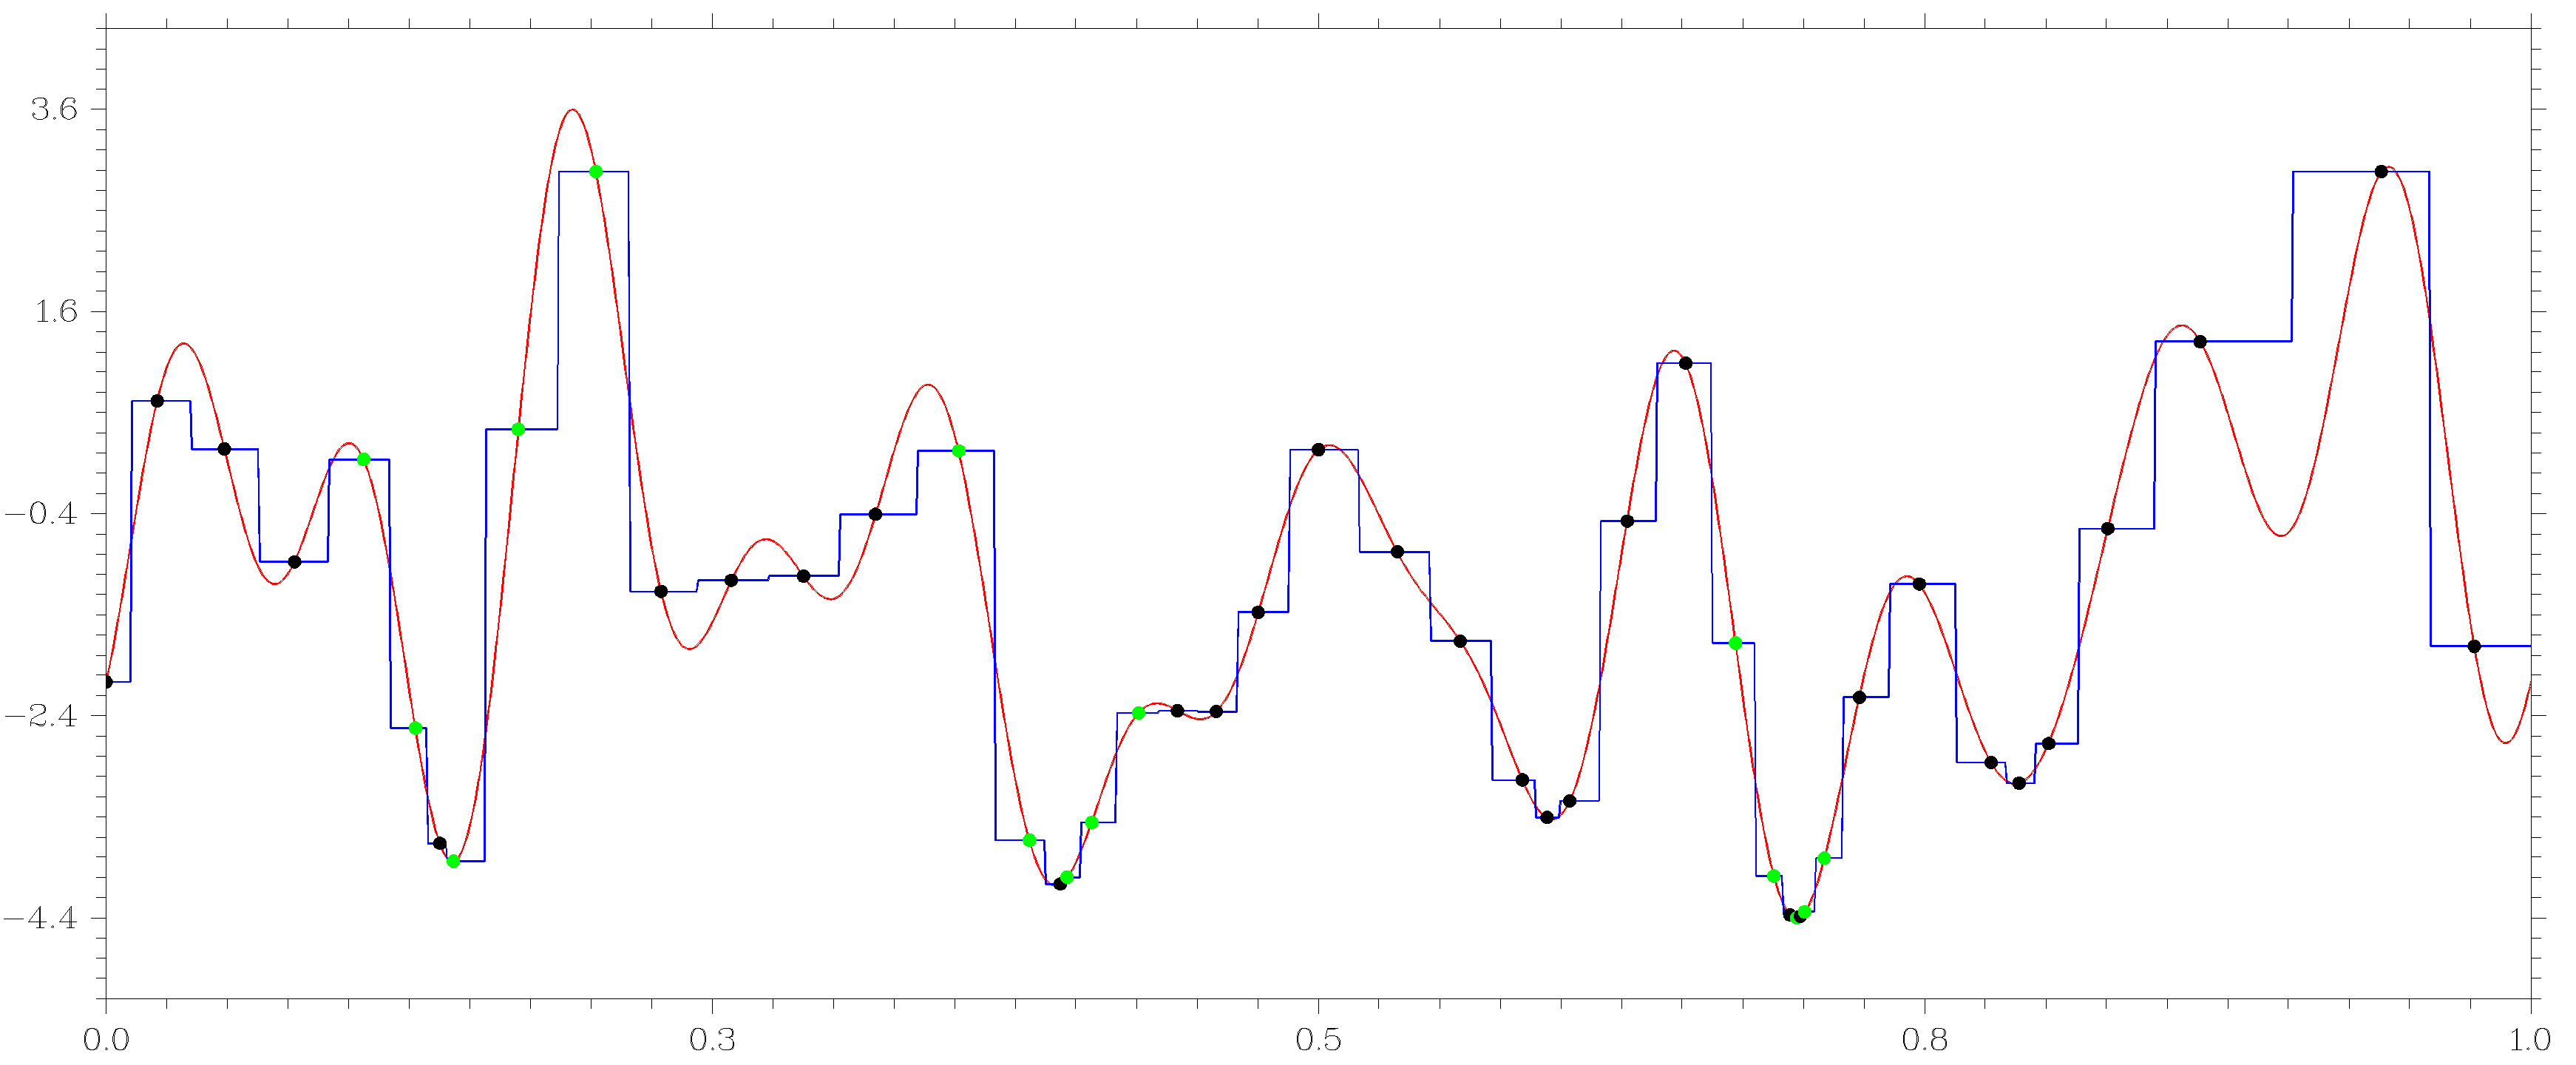
\includegraphics[width=1.0\linewidth]{HillTree90.png}
\caption{Минимизация функции вида (\ref{hill}) с помощью GSA-DT.}
\label{fig2}
\end{figure}   


\subsection{Адаптивная схема редукции размерности }

Рекурсивная схема вложенной оптимизации основана на известном соотношении \cite{Grishagin2001} 
\begin{equation}\label{nested}
\min_{y \in D}\varphi(y) = \min_{y_1\in\left[a_1,b_1\right]}\min_{y_2\in\left[a_2,b_2\right]}...\min_{y_N\in\left[a_N,b_N\right]}\varphi(y),
\end{equation}
которое позволяет свести решение исходной многомерной задачи (\ref{main_problem}) к решению семейства рекурсивно связанных одномерных подзадач.

Для формального описания nested optimization scheme введем семейство функций, определяемых в соответствии с соотношениями 
\begin{equation}\label{nested_N}
\varphi_N(y_1,...,y_N) \equiv \varphi(y_1,...,y_N),
\end{equation}
\begin{equation}\label{nested_i}
\varphi_i(y_1,...,y_i) = \min_{ y_{i+1} \in\left[a_{i+1},b_{i+1}\right]} \varphi_{i+1}(y_1,...,y_i,y_{i+1}), 1\leq i\leq N-1.
\end{equation}

Тогда, в соответствии с (\ref{nested}), для решения многомерной задачи (\ref{main_problem}) достаточно решить одномерную задачу  
\begin{equation}\label{nested_1}
\varphi^* = \min_{y_1\in\left[a_1,b_1\right]}\varphi_1(y_1).
\end{equation}
Однако каждое вычисление значения функции $\varphi_1$ в некоторой фиксированной точке $y_1$ предполагает решение одномерной задачи оптимизации второго уровня 
\begin{equation}
\varphi_1(y_1) = \min_{y_2\in\left[a_2,b_2\right]}\varphi_2(y_1,y_2).
\end{equation}
Вычисление значений функции $\varphi_2$ в свою очередь требует одномерной минимизации функции $\varphi_3$ и т.д. вплоть до решения задачи
\begin{equation}
\varphi_{N-1}(y_1,...,y_{N-1}) = \min_{ y_{N} \in\left[a_{N},b_{N}\right]} \varphi_{N}(y_1,...,y_{N})
\end{equation}
на последнем уровне рекурсии.

Решение возникающего в схеме вложенной оптимизации множества подзадач (\ref{nested_i}) может быть организовано различными способами. 
Очевидный способ (детально проработанный в \cite{Grishagin2001,Grishagin2015} основан на решении подзадач в соответствии с рекурсивным порядком их порождения. Однако здесь возникает потеря значительной части информации о целевой функции. 

Иным  подходом является адаптивная схема, в которой все подзадачи решаются одновременно, что позволяет более полно учитывать информацию о многомерной задаче и за счет этого ускорять процесс ее решения.
Данный подход был теоретически обоснован и апробирован в \cite{Grishagin2016,Grishagin2016_1,Grishagin2018}. 

Кратко отметим, что в рамках исходной схемы вложенной оптимизации порождаемые подзадачи решаются строго последовательно; получаемая в результате иерархическая схема порождения и решения подзадач имеет вид дерева. Построение этого дерева происходит динамически в процессе решения исходной задачи (\ref{main_problem}). При этом вычисление одного значения функции $\varphi_i(y_1,y_2,...,y_i)$ на $i$-м уровне требует полного решения всех задач одного из поддеревьев уровня $i+1$.

Adaptive nested optimization scheme  редукции размерности изменяет порядок решения подзадач: они будут решаться не по одной (в соответствии с их иерархией в дереве задач), а одновременно, т.е. будет существовать некоторое множество подзадач, находящихся в процессе решения. В рамках адаптивной схемы:
\begin{itemize}
	\item 
для вычисления значения функции $i$-го уровня из (\ref{nested_i}) порождается новая задача уровня $i+1$, в которой проводится только одно испытание, после чего новая порожденная задача включается в множество уже имеющихся задач, подлежащих решению;
	\item 
	итерация глобального поиска состоит в выборе одной (наиболее перспективной) задачи из множества имеющихся задач, в которой проводится одно испытание; точка проведения нового испытания определяется в соответствии с базовым алгоритмом глобального поиска из subsection \ref{CoreGSA} или же модифицированным алгоритмом из subsection \ref{TreeGSA};
	\item
в качестве минимальных значений функций из (\ref{nested_i}) используются их текущие оценки, полученные на основе накопленной поисковой информации.
\end{itemize}

Краткое описание основных шагов адаптивной схемы редукции размерности состоит в следующем.

Пусть вложенные подзадачи вида (\ref{nested_i}) решаются с помощью алгоритма глобального поиска, описанного в subsection \ref{CoreGSA}. Тогда каждой подзадаче (\ref{nested_i}) можно присвоить некоторое числовое значение, называемое характеристикой этой задачи. В качестве такой характеристики можно взять значение $R(t)$ из (\ref{MaxR}), т.е. максимальную характеристику из характеристик интервалов, сформированных в данной задаче. Чем выше значение данной характеристики, тем более перспективной является подзадача для продолжения поиска в ней глобального минимума исходной задачи (\ref{main_problem}). Поэтому на каждой итерации выбирается подзадача с максимальной характеристикой для проведения в ней очередного испытания. Это испытание либо приводит к вычислению значения целевой функции $\varphi(y)$ (если выбранная подзадача принадлежала уровню $j=M$), либо порождает новые подзадачи согласно (\ref{nested_i}) при $j\leq M-1$. В последнем случае новые порожденные задачи добавляются к текущему множеству задач, вычисляются их характеристики и процесс повторяется. Завершение процесса оптимизации происходит, когда в корневой задаче выполняется условие остановки алгоритма, решающего эту задачу.



\section{Experimental Results}

Numerical experiments were performed on the Lobachevsky supercomputer of the University of Nizhni Novgorod (operating system -- CentOS 6.4, management system -- SLURM). One supercomputer node has 2 Intel Sandy Bridge E5-2660 2.2 GHz processors, 64 Gb RAM. The CPU is 8-core (i.e. a total of 16 CPU cores are available on the node).

Традиционный подход к оценке эффективности методов глобальной оптимизации основан на численном решении этими методами серии задач из некоторого класса. 
При этом подразумевается, что очередная решаемая задача генерируется посредством некоторого алгоритма.
Типичными примерами таких классов тестовых функций являются функции  Шекеля и Хилла. 
Первый из них (обозначит его $F_{SH}$) основан на формуле 
\begin{equation}\label{shekel}
  \varphi(x)=-\sum_{j=1}^{10}\frac{1}{(K_j(x-A_j)^2+C_j)},\;  x\in[0,10],
\end{equation}
где параметры $1\le K_j\le 3,\: 0 < A_j,\: C_j < 10, \;$ являются независимыми случайными величинами, равномерно распределенными в указанных интервалах.
Следующий генератор (обозначим его $F_{HL}$) определяется выражением
\begin{equation}\label{hill}
  \varphi(x)=\sum_{j=1}^{14}(A_j\sin(2j\pi x) + B_j\cos(2j\pi x)),\: x\in[0,1]
\end{equation}
где значения параметров  $A_j,\: B_j,\: 1 \le j \le 14$, независимо и равномерно распределены в интервале $[-1 ,1 ]$. 

Проведем сравнение базового global search algorithm (GSA) и его модификации, использующей деревья решений (GSA-DT), c известным алгоритмом глобальной оптимизации DIRECT \cite{Jones2009}. Сравнение методов будем проводить при решении 1000 задач из классов $F_{SH}$ и $F_{HL}$. 

Задачу будем считать решенной корректно в случае, если после остановки метода по точности (т.е. когда длина текущего поискового интервала станет меньше $\epsilon$) текущая оценка оптимума $x_k^*$ будет лежать в $\epsilon$-окрестности известного решения задачи $x^*$, т.е. будет выполняться условие $|x^*-x_k^*| \leq \epsilon$.

В таблицах \ref{table:average_Shekel} и \ref{table:average_Hill} приведено число поисковых испытаний, которые в среднем требовалось для минимизации функций Шекеля и Хилла с разной точностью поиска. При этом в скобках в таблице указано число нерешенных задач.

Результаты экспериментов показывают, что при грубой точности решения задачи все методы показывают схожие результаты по числу trials, тогда как при высокой точности решения  алгоритму GSA-DT требуется в 2 раза меньше trials, чем его прототипу. Одновременно GSA-DT превосходит метод DIRECT как по среднему числу search trials, так и по числу корректно решенных задач. В частности, если использовать точность $\epsilon = 10^{-2}$, то метод DIRECT останавливается слишком рано, и не находит глобального решения во многих задачах. 
Поэтому в дальнейших экспериментах, в которых решаются многомерные задачи, мы не будем использовать DIRECT для сравнения, т.к. при решении многомерных задач с остановкой по точности данный метод обеспечиват корректное решение не более чем $50\%$ задач. 

\begin{specialtable}[H] 
	\caption{Среднее число испытаний при минимизации Shekel test functions}\label{table:average_Shekel}
	\center
\begin{tabular}{cccc}
\toprule
        & \textbf{$\epsilon = 10^{-4}$} & \textbf{$\epsilon = 10^{-3}$} & \textbf{$\epsilon = 10^{-2}$} \\
\midrule													
DIRECT         & 64(1) &  34(6)   & 20(17)    \\
GSA            & 106  & 53  &  31   \\ 
GSA-DT         & 49   & 43  &  35   \\

\bottomrule
\end{tabular}
\end{specialtable}

\begin{specialtable}[H] 
	\caption{Среднее число испытаний при минимизации Hill test functions}\label{table:average_Hill}
	\center
\begin{tabular}{cccc}
\toprule
        & \textbf{$\epsilon = 10^{-4}$} & \textbf{$\epsilon = 10^{-3}$} & \textbf{$\epsilon = 10^{-2}$} \\
\midrule					  
DIRECT                & 66(12) & 36(31)  & 20(51)  \\
GSA                   & 130    & 75      & 43      \\
GSA-DT                & 64     & 59      & 50      \\
\bottomrule
\end{tabular}
\end{specialtable}

В следующей серии экспериментов решались многомерные задачи. 
Известным генератором тестовых задач многоэкстремальной оптимизации является генератор GLKS \cite{Gaviano2003}. С его помощью можно порождать тестовые функции с заданными свойствами: числом локальных экстремумов, их областями притяжения, точкой глобального минимума и значением целевой функции в ней, и т.д.
Процедура генерирования тестовых функций состоит в переопределении выпуклой квадратичной функции (параболоида) при помощи полиномов. Тестовые функции определяются пятью параметрами:
\begin{itemize}
	\item размерность задачи $N$;
	\item число локальных минимумов $l$;
	\item значение глобального минимума $f^*$;
	\item радиус области притяжения global optimizer $\rho^*$;
	\item расстояние между global optimizer и вершиной параболоида $d^*$.
\end{itemize}
Изменяя указанные параметры, можно создавать тестовые классы с различными свойствами. Например, при фиксированных размерности задачи и числи локальных минимумов более сложный класс может быть сгенерирован путем сужения области притяжения точки глобального минимума или путем увеличения расстояния между этой точкой и вершиной параболоида.
В проведенных экспериментах использовались значения $l=10$, $f^*=-1$, $\rho^*=0.2$ и $d^*=0.9$.


Для примера рассмотрим работу алгоритмов GSA и GSA-DT при решении одной из двумерных задач, порожденных генератором GKLS. 
Линии уровня оптимизируемой функции, изображенные на figures \ref{fig3} и \ref{fig4}, наглядно показывают наличие десяти локальных экстремумов.
При запуске алгоритмов использовались одинаковые параметры: $r=3.0$ из (\ref{R}) и $\epsilon = 10^{-2}$ в критерии остановки метода.
На figures \ref{fig3} и \ref{fig4} точками черного цвета изображены точки search trials, выполненных методами в процессе решения задачи. При этом алгоритму GSA потребовалось 247 испытаний, тогда как алгоритму GSA-DT хватило 138 испытаний. 
Точкой красного цвета на рисунках отмечено точное решение задачи, а точкой желтого цвета - лучшее его приближение, найденное алгоритмом. 
На рисунке \ref{fig4} точками зеленого цвета отмечены испытания, выполненные в рамках локального поиска. 
Наглядно видно, что в методе с использованием деревьев решений для выделения областей притяжения локальных минимумов снимается проблема накопления точек испытаний в районе локальных экстремумов, присущая исходному алгоритму глобального поиска.


\begin{figure}[H]
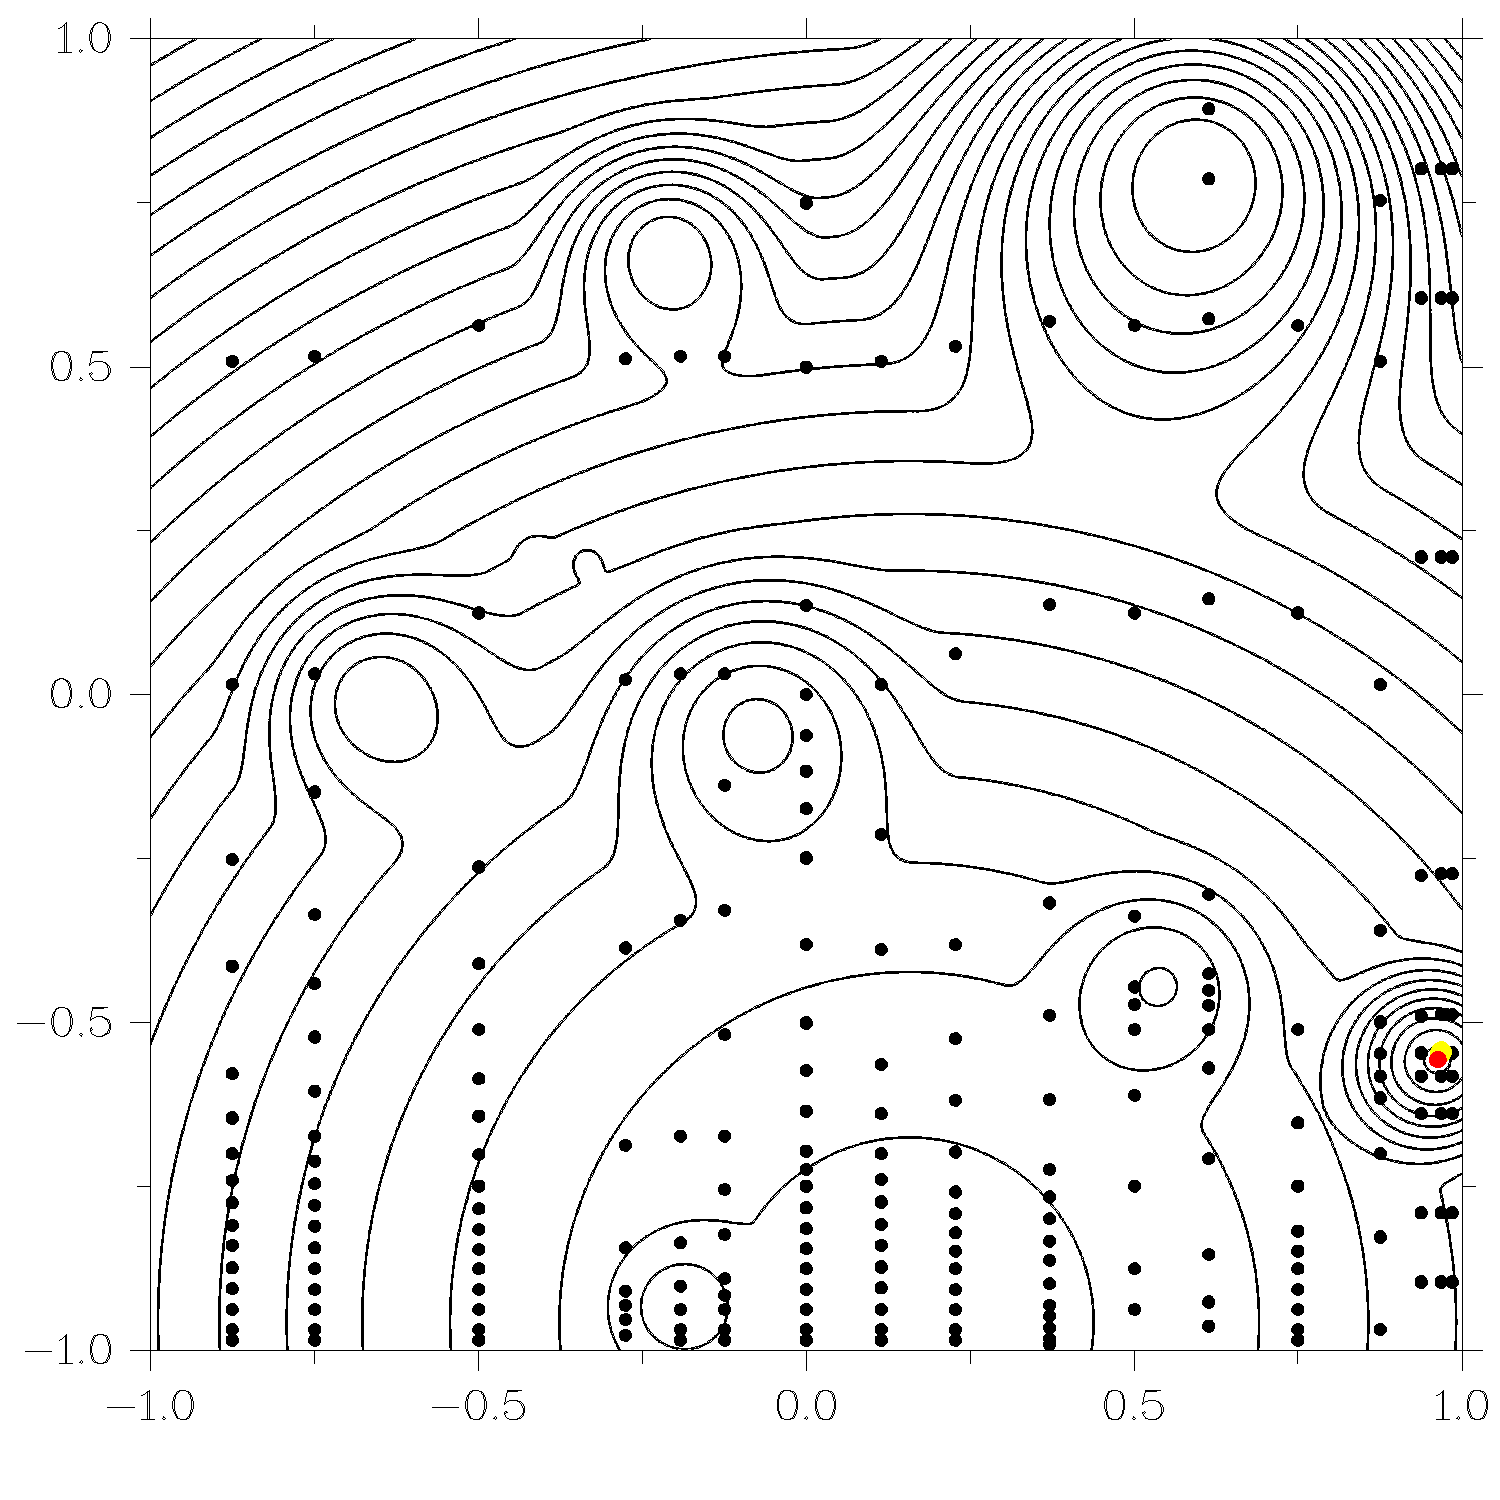
\includegraphics[width=0.6\linewidth]{GKLSAdaptiv6_30line.png}
\caption{Решение задачи GKLS с помощью алгоритма GSA.}
\label{fig3}
\end{figure}   

\begin{figure}[H]
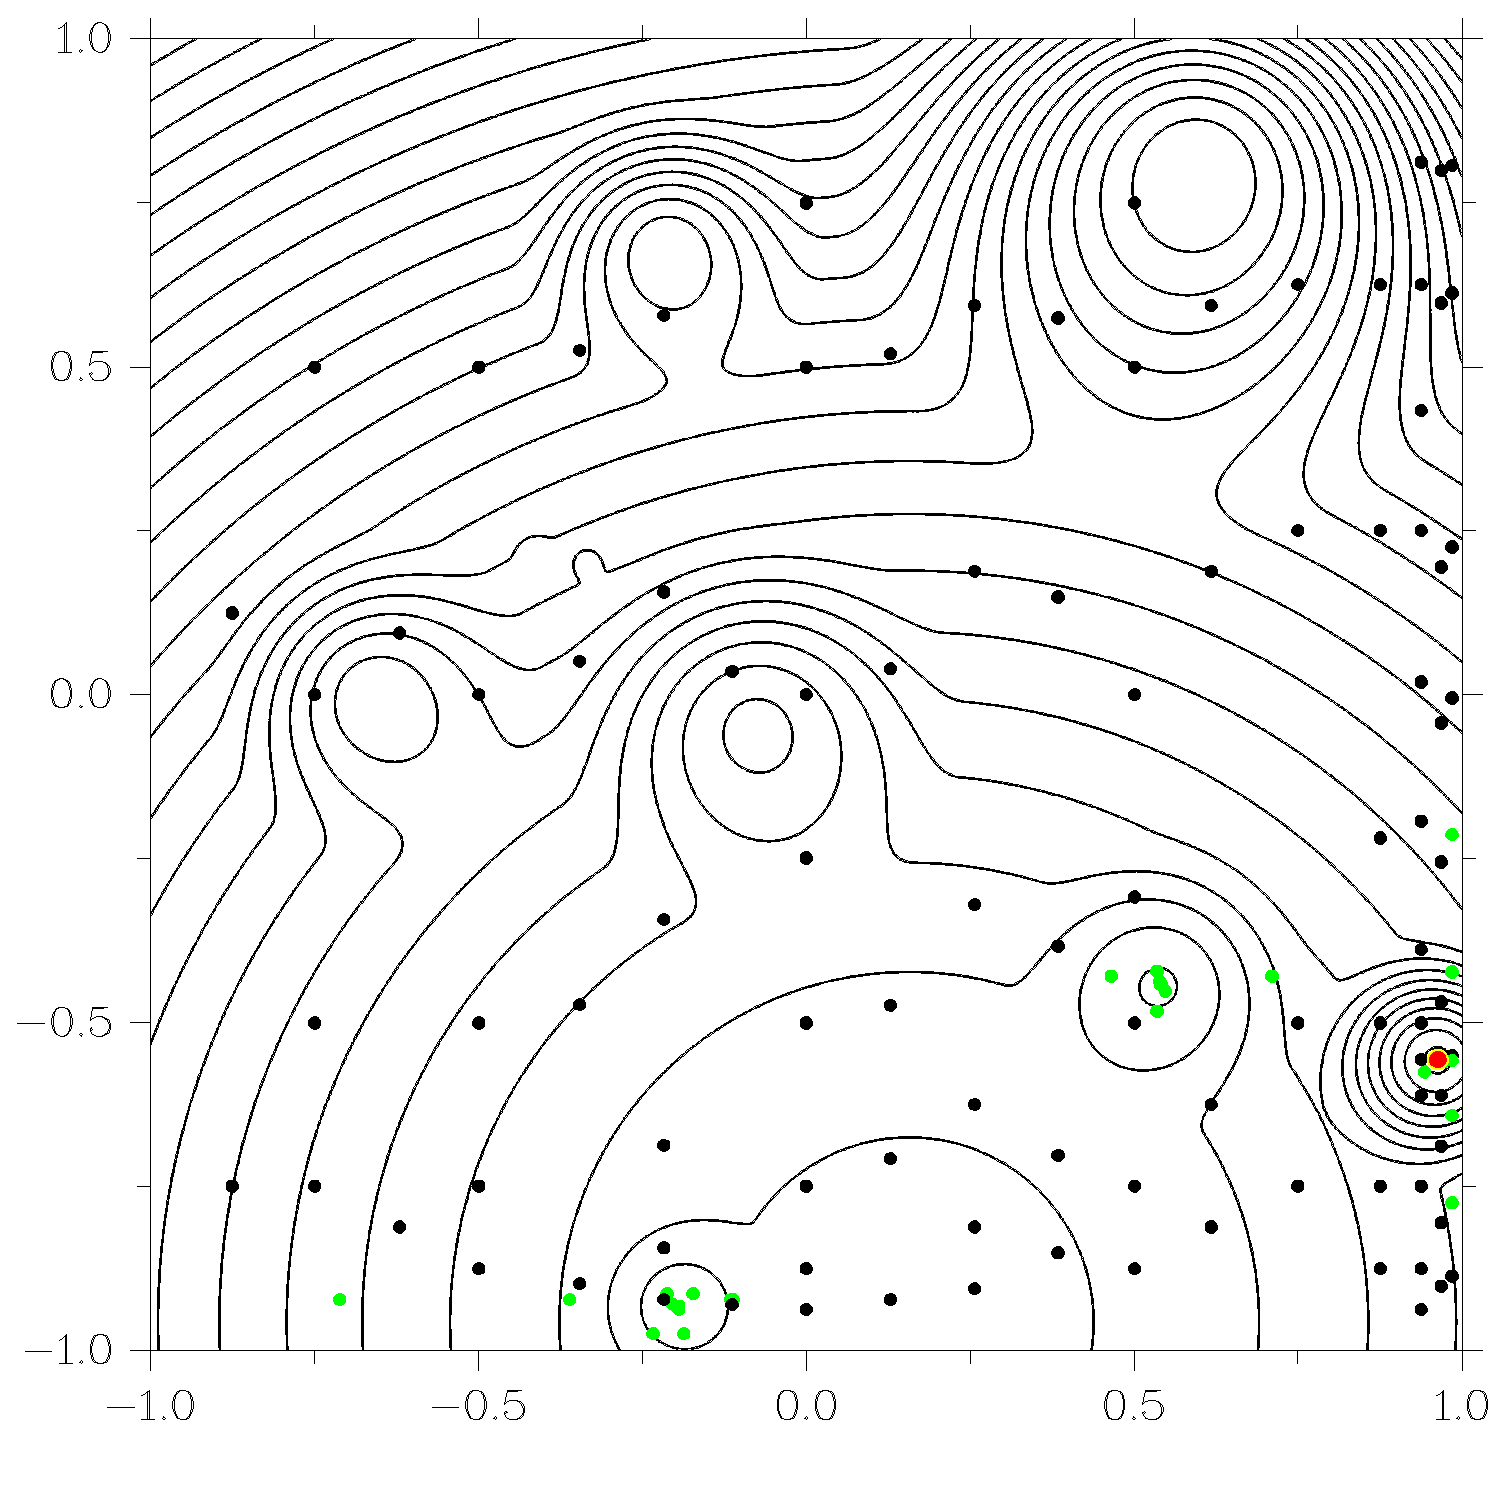
\includegraphics[width=0.6\linewidth]{GKLSTree6_30line.png}
\caption{Решение задачи GKLS с помощью алгоритма GSA-DT.}
\label{fig4}
\end{figure}   

С помощью генератора GKLS было порождено по 300 тестовых задач размерностей $N=2,3,4$ (по 100 задач каждой размерности).
Полученные серии задач были решены с помощью алгоритмов GSA и GSA-DT с параметром $r=5.0$ из (\ref{R}). Указанное значение параметра $r$ обеспечивает решение $100\%$ задач, при меньших значениях параметра некоторые задачи не были решены корректно. Отметим, что метод DIRECT 

В таблицах \ref{table:average_GKLS01} и \ref{table:average_GKLS002} приведено среднее число trials, потребовавшихся методам GSA и GSA-DT для корректного решения всех задач с точностью $\epsilon = 10^{-2}$ и $\epsilon = 2 \cdot 10^{-3}$ соответственно.

Данные из таблиц подтверждают, что алгоритм глобального поиска, использующий выделение локальных экстремумов на основе машинного обучения, обеспечивает более быстрое решение многоэкстремальных задач, чем базовый алгоритм глобального поиска. При решении задач с грубой точностью ускорение составляет порядка $30\%$, тогда как при решении задач с высокой точностью процесс решения ускоряется от 2 до 6 раз. 

\begin{specialtable}[H] 
	\caption{Решение задач GKLS с точностью $\epsilon = 10^{-2}$}\label{table:average_GKLS01}
	\center
\begin{tabular}{cccc}
\toprule
        & $N=2$ & $N=3$  & $N=4$    \\
\midrule
GSA     &  937  &  12716 &  206869  \\
GSA-DT  &  653  &  9204  &  156190  \\
\bottomrule
\end{tabular}
\end{specialtable}

\begin{specialtable}[H] 
	\caption{Решение задач GKLS с точностью $\epsilon = 2 \cdot 10^{-3}$}\label{table:average_GKLS002}
	\center
\begin{tabular}{cccc}
\toprule

       & $N=2$ & $N=3$  & $N=4$    \\
\midrule
GSA    & 1489  & 69764  & 583903  \\
GSA-DT & 831   & 10776  & 173155   \\
\bottomrule
\end{tabular}
\end{specialtable}



%%%%%%%%%%%%%%%%%%%%%%%%%%%%%%%%%%%%%%%%%%
\section{Conclusions}

В статье рассмотрен эффективный детерминированный метод решения задач многоэкстремальной оптимизации -- the information-statistical global search algorithm. 
Для данного алгоритма предложен новый способ ускорения его работы (в терминах числа итераций, требующихся для решения задачи с заданной точностью). Указанный способ основан на выявлении областей притяжения локальных минимумов целевой функции с использованием методов машинного обучения. Выявление областей притяжения и запуск в этих областях локального поиска позволяет существенным образом сократить число испытаний, требующееся методу для достижения глобальной сходимости.  
В рамках исследуемого подхода решение многомерных задач сводится к решению серии информационно-связанных одномерных подзадач, поэтому ключевым моментом является выявление локальных минимумов в одномерных задачах. Для этого используется аппроксимация целевой функции по точкам поисковых испытаний, построенная с помощью деревьев решений. 
Проведены вычислительные эксперименты на серии тестовых задач разной размерности с целью сравнения скорости работы исходного global search algorithm (GSA) и его модификации, которая использует деревья решений для выделения локальных минимумов целевой функции (GSA-DT). 
Результаты экспериментов показывают, что использование алгоритма GSA-DT может значительно (до 6 раз) сократить число испытаний, необходимое для решения задачи с заданной точностью. 

Направлением дальнейших исследований будет использование более сложных моделей целевой фукнции для получения более точной ее аппроксимации. В качестве такого аппроксиматора планируется использовать artificial neural networks. Это потребует разработки новых методов выделения локальных экстремумов, т.к. аппроксимация функции с помощью нейронной сети является более сложной с этой точки зрения. Также планируется уделить внимание вопросам достоверности результатов, полученных с помощью методов машинного обучения. Для решенных модельных задач использование методов машинного обучения показывает хорошие результаты, однако вопрос о том, сохранится ли этот эффект в более сложных задачах, остается открытым. 



%%%%%%%%%%%%%%%%%%%%%%%%%%%%%%%%%%%%%%%%%%
%\section{Patents}

%This section is not mandatory, but may be added if there are patents resulting from the work reported in this manuscript.

%%%%%%%%%%%%%%%%%%%%%%%%%%%%%%%%%%%%%%%%%%
\vspace{6pt} 

%%%%%%%%%%%%%%%%%%%%%%%%%%%%%%%%%%%%%%%%%%
%% optional
%\supplementary{The following are available online at \linksupplementary{s1}, Figure S1: title, Table S1: title, Video S1: title.}

% Only for the journal Methods and Protocols:
% If you wish to submit a video article, please do so with any other supplementary material.
% \supplementary{The following are available at \linksupplementary{s1}, Figure S1: title, Table S1: title, Video S1: title. A supporting video article is available at doi: link.} 

%%%%%%%%%%%%%%%%%%%%%%%%%%%%%%%%%%%%%%%%%%
\authorcontributions{Conceptualization and methodology, K.B.; software and validation, I.L.; formal analysis, K.B.; investigation, I.L.; data curation, I.L.; writing---original draft preparation, K.B.; writing---review and editing, K.B.; visualization, I.L.; funding acquisition, K.B. All authors have read and agreed to the published version of the manuscript.}

\funding{This research was funded by the Ministry of Science and Higher Education of the Russian Federation, agreement number 075-15-2020-808.}

\institutionalreview{Not applicable.}

\informedconsent{Not applicable.}

%\dataavailability{In this section, please provide details regarding where data supporting reported results can be found, including links to publicly archived datasets analyzed or generated during the study. Please refer to suggested Data Availability Statements in section ``MDPI Research Data Policies'' at \url{https://www.mdpi.com/ethics}. You might choose to exclude this statement if the study did not report any data.} 

%\acknowledgments{In this section you can acknowledge any support given which is not covered by the author contribution or funding sections. This may include administrative and technical support, or donations in kind (e.g., materials used for experiments).}

\conflictsofinterest{The authors declare no conflict of interest.} 

%% Optional
%\sampleavailability{Samples of the compounds ... are available from the authors.}

%%%%%%%%%%%%%%%%%%%%%%%%%%%%%%%%%%%%%%%%%%
%% Only for journal Encyclopedia
%\entrylink{The Link to this entry published on the encyclopedia platform.}

%%%%%%%%%%%%%%%%%%%%%%%%%%%%%%%%%%%%%%%%%%
%% Optional
%\abbreviations{Abbreviations}{
%The following abbreviations are used in this manuscript:\\
%
%\noindent 
%\begin{tabular}{@{}ll}
%MDPI & Multidisciplinary Digital Publishing Institute\\
%DOAJ & Directory of open access journals\\
%TLA & Three letter acronym\\
%LD & Linear dichroism
%\end{tabular}}
%
%%%%%%%%%%%%%%%%%%%%%%%%%%%%%%%%%%%%%%%%%%%
%%% Optional
%\appendixtitles{no} % Leave argument "no" if all appendix headings stay EMPTY (then no dot is printed after "Appendix A"). If the appendix sections contain a heading then change the argument to "yes".
%\appendixstart
%\appendix
%\section{}
%\subsection{}
%The appendix is an optional section that can contain details and data supplemental to the main text---for example, explanations of experimental details that would disrupt the flow of the main text but nonetheless remain crucial to understanding and reproducing the research shown; figures of replicates for experiments of which representative data are shown in the main text can be added here if brief, or as Supplementary Data. Mathematical proofs of results not central to the paper can be added as an appendix.
%
%\begin{specialtable}[H] 
%%\tablesize{\scriptsize}
%\caption{This is a table caption. Tables should be placed in the main text near to the first time they are~cited.\label{tab2}}
%%\tablesize{} % You can specify the fontsize here, e.g., \tablesize{\footnotesize}. If commented out \small will be used.
%\begin{tabular}{ccc}
%\toprule
%\textbf{Title 1}	& \textbf{Title 2}	& \textbf{Title 3}\\
%\midrule
%Entry 1		& Data			& Data\\
%Entry 2		& Data			& Data\\
%\bottomrule
%\end{tabular}
%\end{specialtable}
%
%\section{}
%All appendix sections must be cited in the main text. In the appendices, Figures, Tables, etc. should be labeled, starting with ``A''---e.g., Figure A1, Figure A2, etc. 

%%%%%%%%%%%%%%%%%%%%%%%%%%%%%%%%%%%%%%%%%%
\end{paracol}
%%%%%%%%%%%%%%%%%%%%%%%%%%%%%%%%%%%%%%%%%%
\reftitle{References}

% Please provide either the correct journal abbreviation (e.g. according to the “List of Title Word Abbreviations” http://www.issn.org/services/online-services/access-to-the-ltwa/) or the full name of the journal.
% Citations and References in Supplementary files are permitted provided that they also appear in the reference list here. 

%=====================================
% References, variant A: external bibliography
%=====================================
\externalbibliography{yes}
\bibliography{bibliography}

%=====================================
% References, variant B: internal bibliography
%=====================================
%\begin{thebibliography}{999}
%% Reference 1
%\bibitem[Author1(year)]{ref-journal}
%Author~1, T. The title of the cited article. {\em Journal Abbreviation} {\bf 2008}, {\em 10}, 142--149.
%% Reference 2
%\bibitem[Author2(year)]{ref-book1}
%Author~2, L. The title of the cited contribution. In {\em The Book Title}; Editor1, F., Editor2, A., Eds.; Publishing House: City, Country, 2007; pp. 32--58.
%% Reference 3
%\bibitem[Author3(year)]{ref-book2}
%Author 1, A.; Author 2, B. \textit{Book Title}, 3rd ed.; Publisher: Publisher Location, Country, 2008; pp. 154--196.
%% Reference 4
%\bibitem[Author4(year)]{ref-unpublish}
%Author 1, A.B.; Author 2, C. Title of Unpublished Work. \textit{Abbreviated Journal Name} stage of publication (under review; accepted; in~press).
%% Reference 5
%\bibitem[Author5(year)]{ref-communication}
%Author 1, A.B. (University, City, State, Country); Author 2, C. (Institute, City, State, Country). Personal communication, 2012.
%% Reference 6
%\bibitem[Author6(year)]{ref-proceeding}
%Author 1, A.B.; Author 2, C.D.; Author 3, E.F. Title of Presentation. In Title of the Collected Work (if available), Proceedings of the Name of the Conference, Location of Conference, Country, Date of Conference; Editor 1, Editor 2, Eds. (if available); Publisher: City, Country, Year (if available); Abstract Number (optional), Pagination (optional).
%% Reference 7
%\bibitem[Author7(year)]{ref-thesis}
%Author 1, A.B. Title of Thesis. Level of Thesis, Degree-Granting University, Location of University, Date of Completion.
%% Reference 8
%\bibitem[Author8(year)]{ref-url}
%Title of Site. Available online: URL (accessed on Day Month Year).
%\end{thebibliography}

% If authors have biography, please use the format below
%\section*{Short Biography of Authors}
%\bio
%{\raisebox{-0.35cm}{\includegraphics[width=3.5cm,height=5.3cm,clip,keepaspectratio]{Definitions/author1.pdf}}}
%{\textbf{Firstname Lastname} Biography of first author}
%
%\bio
%{\raisebox{-0.35cm}{\includegraphics[width=3.5cm,height=5.3cm,clip,keepaspectratio]{Definitions/author2.jpg}}}
%{\textbf{Firstname Lastname} Biography of second author}

% The following MDPI journals use author-date citation: Arts, Econometrics, Economies, Genealogy, Humanities, IJFS, JRFM, Laws, Religions, Risks, Social Sciences. For those journals, please follow the formatting guidelines on http://www.mdpi.com/authors/references
% To cite two works by the same author: \citeauthor{ref-journal-1a} (\citeyear{ref-journal-1a}, \citeyear{ref-journal-1b}). This produces: Whittaker (1967, 1975)
% To cite two works by the same author with specific pages: \citeauthor{ref-journal-3a} (\citeyear{ref-journal-3a}, p. 328; \citeyear{ref-journal-3b}, p.475). This produces: Wong (1999, p. 328; 2000, p. 475)

%%%%%%%%%%%%%%%%%%%%%%%%%%%%%%%%%%%%%%%%%%
%% for journal Sci
%\reviewreports{\\
%Reviewer 1 comments and authors’ response\\
%Reviewer 2 comments and authors’ response\\
%Reviewer 3 comments and authors’ response
%}
%%%%%%%%%%%%%%%%%%%%%%%%%%%%%%%%%%%%%%%%%%
\end{document}

